% $Header: /cvsroot/latex-beamer/latex-beamer/solutions/generic-talks/generic-ornate-15min-45min.de.tex,v 1.4 2004/10/07 20:53:08 tantau Exp $

\documentclass{beamer}

% Diese Datei enthält eine Lösungsvorlage für:


% - Vorträge über ein beliebiges Thema.
% - Vortragslänge zwischen 15 und 45 Minuten.
% - Aussehen des Vortrags ist verschnörkelt/dekorativ.



% Copyright 2004 by Till Tantau <tantau@users.sourceforge.net>.
%
% In principle, this file can be redistributed and/or modified under
% the terms of the GNU Public License, version 2.
%
% However, this file is supposed to be a template to be modified
% for your own needs. For this reason, if you use this file as a
% template and not specifically distribute it as part of a another
% package/program, I grant the extra permission to freely copy and
% modify this file as you see fit and even to delete this copyright
% notice.



\mode<presentation>
{
  \usetheme{default}
  \setbeamertemplate{frametitle}[default][center]
  \useinnertheme{circles}
  % or ...

  \setbeamercovered{transparent}
  % or whatever (possibly just delete it)
}

\usepackage{url}
\usepackage{color}
%\definecolor{MyLightGrey}{rgb}{0.95,0.95,0.95}
\definecolor{LightGray}{gray}{0.95}

\usepackage[english]{babel}
\usepackage[utf8]{inputenc}
% oder was auch immer

\usepackage{times}
\usepackage[T1]{fontenc}
\usepackage{xspace}
\usepackage{url}
% Oder was auch immer. Zu beachten ist, das Font und Encoding passen
% müssen. Falls T1 nicht funktioniert, kann man versuchen, die Zeile
% mit fontenc zu löschen.

\newcommand{\caret}{\symbol{94}}
\newcommand{\blank}{\symbol{32}}
\newcommand{\mytilde}{\symbol{126}}
\newcommand{\fat}[1]{\mbox{\boldmath $ #1 $}}
\newcommand{\myarcsec}{\hbox{$.\!\!^{\prime\prime}$}}
\newcommand{\myarcmin}{\hbox{$.\!\!^{\prime}$}}
\newcommand{\git}{\texttt{git}\xspace}
\newcommand{\svn}{\texttt{svn}\xspace}
\newcommand{\cvs}{\texttt{cvs}\xspace}
\newcommand{\github}{\texttt{github}\xspace}
\newcommand{\bitbucket}{\texttt{bitbucket}\xspace}

\title[] % (optional, nur bei langen Titeln nötig)
{Source / Version Control \\
Version control systems (\cvs, \svn, \git) \\
Version control hosts (bitbucket, github)}

\author[Thomas Erben] % (optional, nur bei vielen Autoren)
{Thomas Erben, Argelander-Institut f\"ur Astronomie}
% - Der \inst{?} Befehl sollte nur verwendet werden, wenn die Autoren
%   unterschiedlichen Instituten angehören.

\institute[] % (optional, aber oft nötig)
% - Der \inst{?} Befehl sollte nur verwendet werden, wenn die Autoren
%   unterschiedlichen Instituten angehören.
% - Keep it simple, niemand interessiert sich für die genau Adresse.

\date[]{Python lecture on 04/07/2018}

\begin{document}

\begin{frame}
  \titlepage
\end{frame}
%
\begin{frame}
\frametitle{The context - Why Version Control?}
  \centerline{
\includegraphics[height=0.75\textheight]{images/phd101212s}}
\end{frame}
%
\begin{frame}
\frametitle{What is Version Control?}
\small
{\color{red} Program development cycle:}\\
first {\color{blue} revision} $\rightarrow$ bug fixes (second revision)
$\rightarrow$ extensions (third revision) $\rightarrow$ change of
numerical methods (fourth revision) $\rightarrow$ bug fixes ........

\vspace{0.3cm}
{\color{red} Typical sitouations to handle:}
\begin{itemize}
\item I have created some data/made some simulations. With what revision of my
program did I create this?
\item Last year my program gave some result. With the current version
I get something different. What exactly did I change?
\item I need to regenerate a product from last year!
\item I want to change my program but I would like to do this with an old
revision.
\end{itemize}
When you are taking measures to meet these sitouations you are doing
{\color{blue} Version Control}. \cvs, \svn or \git can help you with that.
\end{frame}
%
\begin{frame}
\frametitle{Some terminology}
\small
\begin{itemize}
\item Version control
\item Version control system: \cvs, \svn, \git. For one-person projects it
  does not matter too much which one you use. For collaboration
  efforts \git is definitely the best!
\item repository: \cvs and \svn store the codes in special directories
  on your computers. You can tar these and ship them around.
\item Version control host: \git is optimised for Web based usage and
  cloud services (\github and \bitbucket). Cloud services are
  typically free for public projects!
\end{itemize}
\end{frame}
%
\begin{frame}[fragile]
\frametitle{Poor mans version control}
\small
\begin{verbatim}
user$ ls
calc.c    main.c    README
user$ mkdir safe_29082013
user$ cp *.c README safe_29082013
\end{verbatim}

\alert{Idea:} \\
Create a snapshot from a stable, well-tested program version
(before an important production run; for release purposes; .....)

\vspace{0.2cm}
This is an \emph{important} aspect of Version Vontrol and its most
basic idea!

\vspace{0.2cm}
The poor mans approach becomes unfeasible for larger projects, to
keep a \emph{detailed} history of your development, to easily find
code differences between 01/02/2005 and 29/10/2012, .....!
\end{frame}
%
\begin{frame}[fragile]
\frametitle{Work-cycle under Version Control}
Examples for \cvs with single-user development.
%
\begin{enumerate}
\item You put existing source code under a VCS (\cvs or \svn
  repository, \github upload)
\item check out the code from the VCS
\item \label{enum:modify} modify code, check differences, create
  branches, tag versions, .....
\item check a new revision into the VCS (\textit{commit}; develop a habit on
  \emph{when} to do this!)
\item Go back to \ref{enum:modify} or check out code on another system ....
\end{enumerate}
More steps are necessary for collaboration work under a VCS (e.g.
verify whether a collaborator checked in something new etc.).

There is an additional layer for web-based VCS hosting systens
(\github; local and remote checkins!).
\end{frame}
%
\begin{frame}[fragile]
\frametitle{What are branches?}
\small
You often would like to \textit{branch off} from your main development
trunk:

\vspace{0.2cm}
\centerline{\fbox{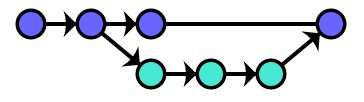
\includegraphics[width=0.5\textwidth]{images/branch}}}
%
\begin{itemize}
\item You want to branch off production code from new developments.
\item You want to create a \textit{sandbox} for new developments
\item You want to provide bug fixes for old releases.
\item Branching is great to allow code verification \textit{before}
  merging new developments to the (stable) main trunk.
\item Branching is the way to contribute to open source projects!
\end{itemize}
Branches are often \emph{merged} to the main development trunk after
some time. Also ideas that do not work out just can be deleted without
harming the main branch!
\end{frame}
%
\begin{frame}
\frametitle{Further Characteristics of Version Control \\ Outlook}
%
\small
\alert{You should put ALL your codes and code related documents under VCS!}
\begin{itemize}
\item You can get version/revision information into your source codes
\item It enforces a certain degree of documentation (commit messages)
\item It can give free secure backup of source codes in addition (cloud services
  such as \github and \bitbucket; \github gives free private repositories
  to academia!)
\item It allows great code-writing in collaborations (private
  projects, Open Source projects; \bitbucket, \github); \alert{No need to work
  in a lock-file mode}; Version Control
  does not substitute communication!
\item It is useful for \emph{all} kind of source code, e.g. also for
  \LaTeX{} files (thesis, science-papers etc.)
\item {\color{red} YOU DETERMINE THE DEGREE OF CONTROL}. You need to
  develop habits for it!
\end{itemize}
\end{frame}
%
\end{document}

%%% Local Variables:
%%% mode: latex
%%% ispell-local-dictionary: "british"
%%% End:
